% -*- program: xelatex -*-
\documentclass[11pt, compress]{beamer}
%\usepackage{listings}

\usepackage{pgfpages}

%\documentclass{article}
%\usepackage{beamerarticle}

%\documentclass[12pt, compress]{beamer} 
%\documentclass[notes=only]{beamer}

\usepackage{fontspec}

\setsansfont{PT Sans}
\setmonofont{PT Mono}

\usepackage{beamerthemesplit}
\usefonttheme[onlymath]{serif}
%\DeclareFontEncoding{T1}
\fontencoding{T1}

%\usepackage[T2A]{fontenc}
%\usepackage[utf8]{inputenc}
\usepackage[russian]{babel}
\usepackage{listings}


\usepackage{amsmath,amssymb,amsthm}
\hypersetup{unicode=true}

\usepackage{color}
\definecolor{mygred}{RGB}{150,0,0} 
\definecolor{mygreen}{RGB}{28,172,0} 
\definecolor{mylilas}{RGB}{170,55,241}
\definecolor{codecolor}{RGB}{0,120,0}
\definecolor{emphcolor}{RGB}{0,0,120}
\definecolor{gray}{RGB}{150,150,150}

\definecolor{light-gray}{gray}{0.95}
\definecolor{light-green}{rgb}{0.93, 1, 0.8}
\definecolor{light-yellow}{rgb}{1,1,0.85}
\definecolor{light-red}{rgb}{0.8, 0.3, 0.3}

\definecolor{dark-blue}{rgb}{0,0,0.6}
\definecolor{dark-red}{rgb}{0.7,0.0,0.0}
\definecolor{dark-green}{RGB}{10,150,0}

\usepackage{pifont}% http://ctan.org/pkg/pifont
\newcommand{\cmark}{\textcolor{green}{\ding{51}}}
\newcommand{\xmark}{\textcolor{red}{\ding{55}}}

\newcommand{\matcode}[1]{ \textcolor{codecolor}{\texttt{#1}}}
\usepackage{graphics,graphicx}
\usepackage{verbatim}
\usepackage{fancyvrb}
\usepackage{booktabs}
%\usepackage{media9}

\usepackage[super]{natbib}
 
\newcommand{\cleartitlepage}[1]{\begin{frame}[plain]\begin{center}\textsc{#1}\end{center}\end{frame}}

\renewcommand{\emph}[1]{\textcolor{emphcolor}{#1}}
\newcommand{\emphb}[1]{\textcolor{emphcolor}{\textbf{#1}}}


\usetheme{CambridgeUS}
\usecolortheme{lily}

\usepackage{tikz}
\usetikzlibrary{positioning} 
\tikzset{cbutton/.style={rectangle,minimum width=10mm,thick,draw=red!50!black!50,
top color=white,bottom color=red!50!black!30}}
\tikzset{mbutton/.style={rectangle,minimum width=10mm,thick,draw=black!20,
top color=white,bottom color=black!30}}


\lstset{basicstyle=\ttfamily\footnotesize,
    language=Python,    
    keepspaces=true,
    extendedchars=true,
    basicstyle={\footnotesize  \color{black}},
    breaklines=true,    
    keywordstyle=\color{blue},
    morekeywords=[2]{1}, keywordstyle=[2]{\color{codecolor}},
    identifierstyle={ \bf \color{black} },
    stringstyle=\color{mylilas},
    commentstyle=\color{mygreen},%
    showstringspaces=false,
    numbers=left,%
    numberstyle={\tiny \color{black}},
    numbersep=7pt, 
    emph=[1]{case,switch,otherwise},emphstyle=[1]\color{blue}, 
    frame=single,    
    rulecolor=\color{red},    
    backgroundcolor=\color{light-gray},
    xleftmargin=0.3cm,
    frame=l,framesep=4pt,framerule=0.5pt,
    showspaces=false,
    escapechar=|
    %lineskip=-0.3pt,
    %emph=[2]{word1,word2}, emphstyle=[2]{style},    
}

\setbeamertemplate{blocks}[rounded][shadow=false]
\setbeamertemplate{navigation symbols}{}

\makeatother
\setbeamertemplate{footline}
{
  \leavevmode%
  \hbox{%
  \begin{beamercolorbox}[wd=.3\paperwidth,ht=2.25ex,dp=1ex,center]{author in head/foot}%
    \usebeamerfont{author in head/foot}\insertshortauthor
  \end{beamercolorbox}%
  \begin{beamercolorbox}[wd=.6\paperwidth,ht=2.25ex,dp=1ex,center]{title in head/foot}%
    \usebeamerfont{title in head/foot}\insertshorttitle
  \end{beamercolorbox}%
  \begin{beamercolorbox}[wd=.1\paperwidth,ht=2.25ex,dp=1ex,center]{date in head/foot}%
    \insertframenumber{} / \inserttotalframenumber\hspace*{1ex}
    %\insertframenumber{} \hspace*{0.1ex}
  \end{beamercolorbox}}%
  \vskip0pt%
}


% define colours
% taken from pickton on Adobe Kuler:
% https://kuler.adobe.com/Some-Kind-Of-Execushares-color-theme-3837185/
 \definecolor{ExecusharesRed}{RGB}{230,37,52}
 \definecolor{ExecusharesBlack}{RGB}{43,40,40}
 \definecolor{ExecusharesBlue}{RGB}{22,190,207}
 \definecolor{ExecusharesWhite}{RGB}{255,255,243}
 \definecolor{ExecusharesGrey}{RGB}{107,110,108}

% \setbeamertemplate{itemize item}{
%  \tikz{
%    \draw[fill=emphcolor,draw=none] (0, 0) rectangle(0.1, 0.1);
%    \draw[fill=emphcolor,draw=none] (0.1, 0.1) rectangle(0.2, 0.2);
%    \draw[fill=emphcolor,draw=none] (0, 0.2) rectangle(0.1, 0.3);
%  }
% }

\AtBeginSection[]{
  \begin{frame}[plain]
  %\vfill  
  \begin{tikzpicture}
  \useasboundingbox (0,0) rectangle(\the\paperwidth,\the\paperheight);  
  \fill[color=mygred]   (-1cm, 3.9cm) rectangle(\the\paperwidth, 5.9cm);
  %\usebeamerfont{title}\insertsectionhead\par%
  %\node[text width=\the\paperwidth,align=center] at (current page.center) {\color{ExecusharesWhite}\Large\textbf{\insertsectionhead}};  
  \node[text width=\the\paperwidth,align=center] at (6cm,4.9cm) {\color{ExecusharesWhite}\Large\textbf{\insertsectionhead}};  
  \end{tikzpicture}
  \end{frame}
}

\setbeamertemplate{headline}{}
\setbeamertemplate{footline}{}

\makeatother
\setbeamertemplate{footline}
{
  \leavevmode%
  \hbox{%  
  \begin{beamercolorbox}[wd=.3\paperwidth,ht=2.25ex,dp=1ex,center]{author in head/foot}%
    \usebeamerfont{author in head/foot}\insertshortauthor
  \end{beamercolorbox}%  
  \begin{beamercolorbox}[wd=.6\paperwidth,ht=2.25ex,dp=1ex,center]{title in head/foot}%
    \usebeamerfont{title in head/foot}\insertshorttitle
  \end{beamercolorbox}%
  \begin{beamercolorbox}[wd=.1\paperwidth,ht=2.25ex,dp=1ex,center]{date in head/foot}%
    \insertframenumber{} \hspace*{1ex}
  \end{beamercolorbox}}%
  \vskip0pt%
}

\setbeamercolor{frametitle}{fg=dark-red,bg=gray!10}
\setbeamerfont{title}{series=\bfseries,parent=structure}
\setbeamerfont{frametitle}{series=\bfseries,parent=structure}



\lstset{language=Matlab,    
    keepspaces=true,
    extendedchars=true,
    basicstyle={\footnotesize  \color{black}},
    breaklines=true,
    morekeywords={matlab2tikz},
    keywordstyle=\color{blue},
    morekeywords=[2]{1}, keywordstyle=[2]{\color{codecolor}},
    identifierstyle={ \bf \color{black} },
    stringstyle=\color{mylilas},
    commentstyle=\color{mygreen},%
    showstringspaces=false,
    numbers=left,%
    numberstyle={\tiny \color{black}}, 
    numbersep=7pt, 
    emph=[1]{case,switch,otherwise},emphstyle=[1]\color{blue}, 
    frame=single,    
    %lineskip=-1.0pt,
    %emph=[2]{word1,word2}, emphstyle=[2]{style},    
} 
%\usetikzlibrary{positioning}
\tikzset{cbutton/.style={rectangle,minimum width=10mm,thick,draw=red!50!black!50,
top color=white,bottom color=red!50!black!30}}
\tikzset{mbutton/.style={rectangle,minimum width=10mm,thick,draw=black!20,
top color=white,bottom color=black!30}}

\title{Основы MATLAB}
\subtitle{Функции, ячейки, строки, структуры}
\author[Самарский университет]{Юдинцев В. В.}
\institute[Самарский университет]{Кафедра теоретической механики}

\newcounter{taskcounter}
\newcommand{\task}{\addtocounter{taskcounter}{1}%
\arabic{taskcounter}. }

\lstset{language=Matlab,    
    keepspaces=true,
    extendedchars=true,
    basicstyle={\footnotesize \color{black}},
    breaklines=true,
    escapeinside={(*}{*)},
    morekeywords={matlab2tikz},
    keywordstyle=\color{blue},
    morekeywords=[2]{1}, keywordstyle=[2]{\color{codecolor}},
    identifierstyle={ \bf \color{black} },
    stringstyle=\color{mylilas},
    commentstyle=\color{mygreen},%
    showstringspaces=false,
    numbers=left,%
    numberstyle={\tiny \color{black}},
    numbersep=7pt, 
    emph=[1]{case,switch,otherwise},emphstyle=[1]\color{blue}, 
    frame=single,
    lineskip=-1.0pt,
    %emph=[2]{word1,word2}, emphstyle=[2]{style},    
}


\begin{document}



{
\usebackgroundtemplate{
\includegraphics[width=\paperwidth,height=\paperheight]{back.png}}
\begin{frame}[plain]
\maketitle
\end{frame}
}


%\section[Содержание]{}
\frame{
\frametitle{Содержание}
\tableofcontents
}
%
%
\section{Функции MATLAB}
%
%
\begin{frame}[fragile]{Математические функции}
  \matcode{sin, cos, tan, cot, acos, asin, ...} -- тригонометрические\\
  \matcode{log, log10, log2, exp, sqrt, nthroot(x,n), ...} \\
  \matcode{sign(a)} -- знак числа \matcode{a}: -1, 0, +1. \\
\end{frame}

\begin{frame}[fragile]{Функции округления}  
  \begin{itemize}
    \item К ближайшему к нулю целому: \\
      \matcode{fix(1.8)=1} но \matcode{fix(-1.8)=-1}
    \item К меньшему целому: \\
    \matcode{floor(-1.9)=-2} но \matcode{floor(1.9)=1}
    \item К большему целому: \\
    \matcode{ceil(1.3)=2}
    \item К ближайшему целому: \\
    \matcode{round(1.4)=1}, \matcode{round(-1.5)=-2}
  \end{itemize}
\end{frame}



\begin{frame}[fragile]{Функции комплексных чисел}
  \begin{itemize}
    \item \matcode{abs(z)} -- модуль.
    \item \matcode{angle(z)} -- аргумент.
    \item \matcode{conj(z)} -- комплексно-сопряженное число.
    \item \matcode{imag(z)} -- мнимая часть.
    \item \matcode{real(z)} -- вещественная часть.
    \item \matcode{isreal(z)} -- 1, если z -- вещественное число, 0 -- мнимое.
  \end{itemize}
\end{frame}

\begin{frame}[fragile]{Специальные матрицы}  
  \begin{itemize}
    \item \matcode{eye(n), eye(n,m)} -- единичные матрицы $n \times n$.
\begin{lstlisting}
>> eye(3,4)
ans =
     1     0     0     0
     0     1     0     0
     0     0     1     0  
\end{lstlisting}
    \item \matcode{rand(n), rand(n,m)} -- матрица псевдослучайных чисел
    \item \matcode{ones(n,m)} -- матрица $n \times m$, заполненная единицами
    \item \matcode{zeros(n,m)} -- матрица $n \times m$, заполненная нулями
  \end{itemize}
\end{frame}

\begin{frame}[fragile]{Специальные матрицы}  
\matcode{magic(n)} -- квадратная матрица $n \times n$,с одинаковыми суммами элементов по строкам и столбцам и диагоналям.
\begin{lstlisting}
>> magic(3)
ans =
     8     1     6
     3     5     7
     4     9     2
\end{lstlisting}
\end{frame}

\begin{frame}[fragile]{Фунция \emph{size}}  
Количество элементов по каждой размерности (результат -- массив)
\begin{lstlisting}
>> a = [1 2 3; 4 5 6];
>> size(a)

ans = 
    2   3
\end{lstlisting}
Количество элементов по 1 и 2 размерности 
\begin{lstlisting}
>> a = [1 2 3; 4 5 6];
>> size(a,1)

ans = 
    2
>> size(a,2)    

ans = 
    3
\end{lstlisting}
\end{frame}

\begin{frame}[fragile]{Фунция \emph{numel}}  
Количество элементов:
\begin{lstlisting}
>> a = [1 2 3; 4 5 6];
>> numel(a)

ans = 
    6
\end{lstlisting}
\end{frame}

\begin{frame}[fragile]{Функция \emph{reshape}}
Преобразование матрицы-строки 1x6 в матрицу 3x2
\begin{lstlisting}
>> a = [1 2 3 4 5 6];
>> b = reshape(a, 3, 2)

b = 
    1   4
    2   5
    3   6
\end{lstlisting}

Преобразование матрицы-строки 1x6 в матрицу 2x3
\begin{lstlisting}
>> a = [1 2 3 4 5 6];
>> b = reshape(a, 2, 3)

b = 
    1   3   5
    2   4   6  
\end{lstlisting}

\end{frame}  

\begin{frame}[fragile]{Функция \emph{reshape}}
Преобразование матрицы 3x2 в матрицу 2x3
\begin{lstlisting}
>> a = [1  4
        2  5
        3  6];
>> b = reshape(a, 2, 3)

b = 
    1   3   5
    2   4   6 
\end{lstlisting}

\end{frame}  


\begin{frame}[fragile]{Функции над матрицами}
  \begin{itemize}    
    \item \matcode{diag(A), diag(A,k)} -- строка, содержащая диагональные элементы матрицы $\mathbf A$, если $\mathbf A$ - матрица (k=0 для главной диагонали).
    \item \matcode{diag(V)} -- диагональная матрица с элементами вектора $V$ на диагонали, если $V$ - вектор.
    \item \matcode{tril(A), tril(A,k)} -- нижняя  треугольная матрица, построенная по матрице $A$.
    \item \matcode{triu(A), triu(A,k)} -- верхняя треугольная матрица, построенная по матрице $A$.
  \end{itemize}
\end{frame}

\begin{frame}[fragile]{Функции над матрицами}
  Параметр $k$ в функциях \matcode{diag(A,k), tril(A,k), triu(A,k)}
  \begin{figure}[ht]
  \centering
  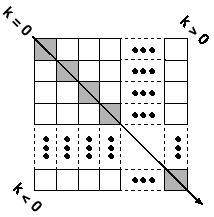
\includegraphics[width=4cm]{./diag.png}
  \end{figure}
\end{frame}

\begin{frame}[fragile]{Функция \emph{repmat}}
\alert{rep}eat \alert{mat}rix -- создать матрицу, используя 2 копии матрицы $a$ по первой размерности и восемь копий матрицы $a$ во второй размерности:
\begin{lstlisting}  
>> a = [1  8];
>> b = repmat(a, 2, 4)

b = 
    1   8   1   8   1   8   1   8 
    1   8   1   8   1   8   1   8 
\end{lstlisting}
\end{frame}

\begin{frame}[fragile]{Векторное произведение}
Векторное произведение строк  
\begin{lstlisting}
>> cross([1,2,3],[4,5,6])
ans =
    -3     6    -3
\end{lstlisting}

Векторное произведение столбцов
\begin{lstlisting}
>> cross([1;2;3],[4;5;6])

ans =
    -3
     6
    -3    
\end{lstlisting}
\end{frame}

\begin{frame}[fragile]{Векторное произведение аргументов-матриц}
Для аргументов-матриц векторное произведение выполняется для векторов, которые расположены по первой размерности, равной 3:  
\begin{lstlisting}
>> a = [1 2 3;
        2 5 6; 
        3 8 9];

>> b = [1 1 3; 
        2 1 3; 
        3 1 2];     

>> cross(a,b)
ans =
     0    -3   -15
     0     6    21
     0    -3    -9
\end{lstlisting}

$$
  c(:,i) = a(:,i) \times b(:,i)
$$
\end{frame}

\begin{frame}[fragile]{Векторное произведение аргументов-матриц}
Третьим аргументом указывается размерность в которой расположены векторы.  
\begin{lstlisting}
>> a = [1 2 3;
        4 5 6; 
        7 8 9];

>> b = [1 2 3; 
        1 2 3; 
        1 2 2];     

>> cross(a,b,2)
ans =
     0     0     0
     3    -6     3
    -2    -5     6
\end{lstlisting}

$$
  c(i,:) = a(i,:) \times b(i,:)
$$
\end{frame}

\begin{frame}[fragile]{Скалярное произведение}
Векторы-строки  
\begin{lstlisting}
>> a = [1 2 3];
>> b = [2 2 2];     
>> dot(a,b)
ans =
    12
\end{lstlisting}
Столбцы и строки
\begin{lstlisting}
>> a = [1; 2; 3];
>> b = [2  2  2];     
>> dot(a,b)
ans =
    12
\end{lstlisting}
\end{frame}

\begin{frame}[fragile]{Скалярное произведение}
При скалярном произведении матриц матрицы перемножаются по первой размерности не равной 1 (матрицы должны быть одинаковых размеров)
\begin{lstlisting}
>> a = [1 2 3;
        4 5 6; 
        7 8 9];

>> b = [1 2 3; 
        1 2 3; 
        1 2 2];     

>> dot(a,b)
ans =
    12    30    45
\end{lstlisting}

$$
  c(:,i) = a(:,i) \cdot b(:,i)
$$
\end{frame}

\begin{frame}[fragile]{Скалярное произведение}
Третьим аргументом можно указать явно размерность, в которой расположены векторы в матрице
\begin{lstlisting}
>> a = [1 2 3;
        4 5 6; 
        7 8 9];

>> b = [1 2 3; 
        1 2 3; 
        1 2 2];     

>> dot(a,b,2)
ans =
    14
    32
    41
\end{lstlisting}
$$
  c(i,:) = a(i,:) \cdot b(i,:)
$$
\end{frame}

\begin{frame}[fragile]{Сумма элементов вектора или матрицы}
  \matcode{sum(a)}

  Сумма элементов вектора:
  \begin{lstlisting}
  >> a=[1 2 3 4];
  >> sum(a)
  ans=
     10     
  \end{lstlisting} 
  Сумма элементов матрицы:
  \begin{lstlisting}
  >> a=[1 2;
        3 4];
  >> sum(a)
  ans=
     4 6     
  \end{lstlisting} 
\end{frame}

\begin{frame}[fragile]{Сумма элементов матрицы}
  Сумма элементов матрицы по заданной размерности:
  \begin{lstlisting}
  >> a=[1 2;
        3 4];
  >> sum(a,2)
  ans =
     3
     7    
  \end{lstlisting} 
\end{frame}


\begin{frame}[fragile]{Сортировка}
\begin{itemize}
  \item \matcode{sort(a)} -- сортировка вектора или матрицы. 
  \item Если \matcode{a} -- матрица, то производится сортировка элементов в столбцах (по первой размерности)
\end{itemize}
\begin{lstlisting}
>> a = magic(3)
a =
  8     1     6
  3     5     7
  4     9     2
>> sort(a)
ans =
  3     1     2
  4     5     6
  8     9     7
\end{lstlisting}
\end{frame}


\begin{frame}[fragile]
\frametitle{Сортировка}
Вторым аргументом функции \matcode{sort} может быть номер измерения, по которому должна выполняться сортировка: 
\begin{lstlisting}
>> a = magic(3)
a =

     8     1     6
     3     5     7
     4     9     2

>> sort(a,2)
ans =

     1     6     8
     3     5     7
     2     4     9
\end{lstlisting}
\end{frame}


\begin{frame}[fragile]{Сортировка}
\matcode{[res,i]=sort(a)}. \matcode{i} содержит индексы элементов исходного вектора \matcode{a}, расположенные по порядку сортировки.
\begin{lstlisting}
>> a = magic(3)
a =
     8     1     6
     3     5     7
     4     9     2
>> [res,i] = sort(a)

res =
     3     1     2
     4     5     6
     8     9     7
i =
     2     1     3
     3     2     1
     1     3     2   
\end{lstlisting}
\end{frame}

\begin{frame}[fragile]{Среднее значение}
\begin{lstlisting}
>> a = [1 2 6]
>> mean(a)
ans = 
     3
\end{lstlisting}
Среднее в столбцах
\begin{lstlisting}
>> a = [1 2 6;
        7 8 9];
>> mean(a)

ans = 
     4   5   6
\end{lstlisting}
Среднее в строках
\begin{lstlisting}
>> mean(a, 2)

ans = 
     2
     8
\end{lstlisting}
\end{frame}

\begin{frame}[fragile]{Максимум}
\begin{lstlisting}
>> a = [1 9 6]
>> max(a)
ans = 
     9
\end{lstlisting}
Максимум из двух массивов
\begin{lstlisting}
>> a = [1 9 6]
>> max(a,2)
ans = 
     [2  9   6]
\end{lstlisting}
\end{frame}

\begin{frame}[fragile]{Максимум}
\begin{lstlisting}
>> a = [1 9 10;
        4 6 1];
>> max(a)
ans = 
     4  9  10
\end{lstlisting}
Размерность, по которой определяется максимум задается третьим аргументом  
\begin{lstlisting}
>> max(a,[],2)
ans = 
     10
     6
\end{lstlisting}
\end{frame}

\begin{frame}[fragile]{Индексы максимальных значений}
\begin{lstlisting}
a = [8     1     6;
     3     5     7;
     4     9     2];
>> [~,i] = max(a)

i =
     1     3     2
\end{lstlisting}
Аналогичным образом работает функция \emph{min}
\begin{lstlisting}
>> a = [1 9 10;
        4 6 1];
>> min(a)
ans = 
     1  6  1
\end{lstlisting}
\end{frame}

\section{Множества}

\begin{frame}[fragile]{Работа с множествами}
  \matcode{intersect(A, B)} -- пересечение векторов А и В как множеств:
\begin{lstlisting}
>> a = [1 2 3 7 8 7 3 1];
>> b = [7 1 5 6];
>> intersect(a,b)
ans =
     1     7 
\end{lstlisting}
\matcode{ismember(A, S)} -- содержит ли А элементы из S:
\begin{lstlisting}
>> a = [1 2 3 7 8 7 3 1];
>> b = [7 1 5 6];
>> ismember(a,b)
ans =
     1     0     0     1     0     1     0     1
\end{lstlisting}
\end{frame}

\begin{frame}[fragile]{Работа с множествами}
  \matcode{setdiff(A, B)} -- элементы, входящие в А, но отсутствующие в В (A-B):
\begin{lstlisting}
>> a = [1 2 3 7 8 7 3 1];
>> b = [7 1 5 6];
>> setdiff(a,b)
ans =
     2     3     8
\end{lstlisting}
  \matcode{setxor(A, B)} -- элементы, не входящие в результат пересечения множеств А и В:
\begin{lstlisting}
>> a = [1 2 3 7 8 7 3 1];
>> b = [7 1 5 6];
>> setdiff(a,b)
ans =
     2     3     5     6     8
\end{lstlisting}
\end{frame}

\begin{frame}[fragile]{Работа с множествами}
  \matcode{union(A, B)} -- объединение множеств:
\begin{lstlisting}
>> a = [1 2 3 7 8 7 3 1];
>> b = [7 1 5 6];
>> union(a,b)
ans =
     1     2     3     5     6     7     8
\end{lstlisting}
  \matcode{unique(A)} -- элементы вектора А без повторений:
\begin{lstlisting}
>> a = [1 2 3 7 8 7 3 1];
>> unique(a)
ans =
     1     2     3     7     8
\end{lstlisting}
\end{frame}

\section{Битовые функции}

\begin{frame}[fragile]{Битовые функции}
  \matcode{bitand(a,b)} -- поразрядное И
\begin{lstlisting}
  >> bitand(5,1)
  ans =
        1
\end{lstlisting}
  \matcode{bitor(a,b)} -- поразрядное ИЛИ
\begin{lstlisting}
  >> bitor(4,2)
  ans =
        6
\end{lstlisting}
  \matcode{bitset(a,bit,v)} -- установка бита в позиции bit числа a; v = 1 или 0
\begin{lstlisting}
  >> bitset(5,3,0)
  ans =
        1
\end{lstlisting}
\end{frame}

\begin{frame}[fragile]{Преобразование числа к другому основанию}  
  \matcode{dec2bin(a)} -- \alert{строка} с двоичным представлением положительного числа $a$
  \begin{lstlisting}
  >> dec2bin(5)
  ans =
      101
  \end{lstlisting}
  \matcode{dec2hex(a)} -- \alert{строка} с шестнадцатеричным представлением положительного числа $a$
  \begin{lstlisting}
  >> dec2hex(255)
  ans =
      FF
  \end{lstlisting}  
\end{frame}

\begin{frame}[fragile]{Преобразование числа к другому основанию}  
\matcode{bin2dec(a)} -- преобразование строки с двоичным представлением числа к десятичной системе $a$
  \begin{lstlisting}
  >> bin2dec('111')
  ans =
      7
  \end{lstlisting}
  \matcode{hex2dec(a)} -- преобразование строки с шестнадцатеричным представлением числа к десятичной системе $a$
  \begin{lstlisting}    
  >> hex2dec('F1')
  ans =
      241    
  \end{lstlisting}
\end{frame}

\section{Ячейки}

\begin{frame}[containsverbatim]{Ячейки}
  Массивы ячеек (cells) могут хранить данные различных типов: числа, строки, структуры, массивы ячеек.
\begin{lstlisting}[frame=single]   
>> data{1} = 'Текст'
data = 
    'Текст'
>> data{2} = 1
data = 
    'Текст'    [1]
>> data{5} = [1 2 3]
data = 
    'Текст'    [1]    []    []    [1x3 double]
\end{lstlisting}
\end{frame}

\begin{frame}[containsverbatim]{Доступ к элементам массива ячеек}
\begin{lstlisting}[frame=single]   
>> data{1}
ans =
     Текст

>> data{2}
ans =
     1

>> data{5}
ans =
     1     2     3
\end{lstlisting}
\end{frame}

\begin{frame}[containsverbatim]{Функция cell}
Формирование пустой матрицы ячеек
\begin{lstlisting}
>> a = cell(3,4)
a = 
    []    []    []    []
    []    []    []    []
    []    []    []    []
\end{lstlisting}    
Присвоение значения элементу новой матрицы 
\begin{lstlisting}
>> a{2,3} = 'элемент 2,3'
a = 
    []    []                      []    []
    []    []    'элемент 2,3'     []
    []    []                      []    []
\end{lstlisting}
\end{frame}

\begin{frame}[fragile]{Функции для работы с ячейками}
\setbeamercovered{transparent}
Преобразование числовой матрицы в матрицу ячеек
\begin{lstlisting}
>> a=magic(5)
a =
    17    24     1     8    15
    23     5     7    14    16
     4     6    13    20    22
    10    12    19    21     3
    11    18    25     2     9
\end{lstlisting}
\pause
\begin{lstlisting}
>> b = mat2cell(a,[2 3],[2 1 2])
b = 
    [2x2 double]    [2x1 double]    [2x2 double]
    [3x2 double]    [3x1 double]    [3x2 double]
\end{lstlisting}
\end{frame}


\begin{frame}[fragile]{Преобразование матрицы ячеек в числовую матрицу}
Функция \matcode{mat2cell}:
\begin{lstlisting}
>> b = mat2cell(a,[2 3],[2 1 2])
b = 
    [2x2 double]    [2x1 double]    [2x2 double]
    [3x2 double]    [3x1 double]    [3x2 double]
>> cell2mat(b)
ans =
    17    24     1     8    15
    23     5     7    14    16
     4     6    13    20    22
    10    12    19    21     3
    11    18    25     2     9
\end{lstlisting}
\end{frame}


\section{Структуры}

\begin{frame}[containsverbatim]{Структура}
Структура -- это элемент данных, который может содержать разнотипные \alert{поля}:
\begin{small}
\begin{Verbatim}[formatcom=\color{codecolor}]
  имя = struct('поле1',значение,'поле2',значение,...)
\end{Verbatim}   
\end{small}
Структура, описывающая параллелепипед:
\begin{lstlisting}[frame=single]
box=struct('height', 100, 'width', 10, 'depth', 5)
box= 
    height: 100
     width: 10
     depth: 5
\end{lstlisting}
\end{frame}

%
%
%

\begin{frame}[fragile]{Доступ к полям структуры}
\begin{itemize}
 \item Считывание значения поля
\begin{lstlisting} 
>> box.height
ans =
   100
\end{lstlisting}
  \item Имя поля может быть задано строкой
\begin{lstlisting}[frame=single]
>> box.('height')
ans =
   100
\end{lstlisting}
\end{itemize}
\end{frame}


\begin{frame}[containsverbatim]{Список полей структуры}
\begin{lstlisting}[frame=single]
>> names = fieldnames(box)
names = 
    'height'
    'width'
    'depth'
    'mass'
\end{lstlisting} 
\end{frame}


\begin{frame}[containsverbatim]{Изменение значения поля}
\begin{lstlisting}[frame=single]
>> box.height = 20
box = 
    height: 20
     width: 10
     depth: 5
\end{lstlisting}
\end{frame}

%
%
%

\begin{frame}[containsverbatim]{Добавление поля}
Для добавления поля к структуре необходимо присвоить значение новому полю, как существующему:
\begin{lstlisting}[frame=single]
>> box.mass=5
box = 
    height: 20
     width: 10
     depth: 5
      mass: 5
\end{lstlisting}
\end{frame}

\begin{frame}[containsverbatim]{Создание структуры}
Cоздание новой структуры без использования функции \matcode{struct}:
\begin{lstlisting}
>> sphere2.radius=2
sphere2 = 
    radius: 2
\end{lstlisting}
\end{frame}

\section{Строки}

\begin{frame}[fragile]
\frametitle{Строковые переменные}
Строки создаются при помощи одинарных кавычек
\begin{lstlisting}
>> a = 'To be or not to be?'
\end{lstlisting}
Строка это массив символов
\begin{lstlisting}
>> whos
  Name         Size       Bytes  Class   Attributes

  a            1x19          38  char    
\end{lstlisting}
\end{frame}


\begin{frame}[fragile]
\frametitle{Склейка строк}
Для склейки двух строк их можно объединить в матрицу-строку:
\begin{lstlisting}
>> S1 = 'String 1 ';
>> S2 = 'String 2';
>> [S1 S2]
ans =

    'String 1 String 2'
\end{lstlisting}
или использовать функцию \matcode{strcat}
\begin{lstlisting}
>> strcat(S1, S2)
ans =

    'String 1String 2'
\end{lstlisting} 
Во втором случае пробелы в конце строк игнорируются.
\end{frame}

\section{Вывод результатов}

\begin{frame}[fragile]  
\frametitle{Функция disp}
Функция \alert{disp} выводит результат с форматированием по умолчанию.  
\begin{lstlisting}
>> a = [1.0 2.5 3.0];
>> disp(a);
    1.0000    2.5000    3.0000

>> disp('Result')    
Result
\end{lstlisting}
Такой же результат можно получить, записав выражение без точки с запятой в конце.
\begin{lstlisting}
>> a = [1.0 2.5 3.0]

a =
    1.0000    2.5000    3.0000
\end{lstlisting}  
\end{frame}

\begin{frame}[fragile]
\frametitle{Функция fprintf}
Функция \alert{fprintf} используется для форматированного вывода:
\begin{lstlisting}
>> a = [1.0 2.5 3.0];
>> fprintf('%3.1f %3.1f %4.2f\n', a);
1.0 2.5 3.00

>> fprintf('%+6.3f\n', 1.5);
+1.500 

>> fprintf('%+6.3f\n', -1.5);
-1.500 

>> fprintf('%+08.3f\n', -1.5);
-001.500 
\end{lstlisting}

\begin{lstlisting}
>> fprintf('%3.1f\n', a);
1.0
2.5
3.0
\end{lstlisting}
\end{frame}

\begin{frame}[fragile]
\frametitle{Функция fprintf}
\begin{lstlisting}
>> fprintf('%+3.3e\n', -1.5);
-1.500e+00

>> fprintf('Square root of %i is %3.1f\n', 4, sqrt(4));
Square root of 4 is 2.0
\end{lstlisting}

Функция \alert{fprintf} может использоваться для записи в файл
\begin{lstlisting}
a = [1 2 3; 4 5 6];  
f = fopen('res.txt','w');  
fprintf(f, '%5.2f %5.2f %5.2f\n', a(1,:));
fprintf(f, '%5.2f %5.2f %5.2f\n', a(2,:));
fclose(f);
\end{lstlisting}


\end{frame}






% %
% %
% %
% %
% \section{Задачи}
% %
% %
% %
% %

% \begin{frame}[c]{Задание 1}
% Напишите кратчайшее однострочное выражение для построения квадратной матрицы вида
%   $$
%   \begin{bmatrix}
%    1 & 2 & 3 & 4 & \ldots & n \\
%    1 & 2 & 3 & 4 & \ldots & n \\
%    \ldots & \ldots & \ldots & \ldots & \ldots & n \\
%    1 & 2 & 3 & 4 & \ldots & n
%   \end{bmatrix}
%   $$
% \end{frame}

% \begin{frame}[c,fragile]{Задание 2}
% Напишите выражение, определяющее индекс элемента вектора с наименьшим отклонением от среднего значения элементов вектора $\mathbf P$
% $$ 
%   i: \text{min }|P_i-m(\mathbf P)|
% $$
% Например, для 
% $$ P = [8,1,2,2,0,3] $$
% ответом будет $6$, т.е. шестой элемент массива находится ближе всего к среднему значению элементов массива. Среднее значение определяется при помощи функции \emphb{mean}
% \begin{lstlisting}
% >> P=[8 1 2 2 0 3];
% >> mean(P)
% ans =  2.6667
% >>
% \end{lstlisting}

% \end{frame}

% \begin{frame}[c]{Задание 3}
% Напишите код, который находит матрицу $\mathbf B$, отличающуюся от матрицы $\mathbf A$ перестановкой столбцов по возрастанию суммы элементов столбца.
% $$
%   \mathbf A = 
%   \begin{bmatrix}
%     2 & 3 & 5 \\
%     4 & 1 & 9 \\
%     3 & 0 & 2
%   \end{bmatrix} \quad \Rightarrow \quad 
%   \mathbf B = 
%   \begin{bmatrix}
%     5 & 2 & 3 \\
%     9 & 4 & 1 \\
%     2 & 3 & 0
%   \end{bmatrix}
% $$
% $$
%   \boxed{5 + 9 + 2} > \boxed{2 + 4 + 3} > \boxed{3 + 1 + 0}
% $$
% \end{frame}


% \begin{frame}[fragile]{Задание 4}
% В матрице $\mathbf A$ записаны координат точек на плоскости: в первом столбце --  координаты $x$, во втором столбце -- $y$:
% $$
%   \boldsymbol A = \begin{bmatrix} x_1 & y_1 \\ x_2 & y_2 \\ x_3 & y_3 \\ \ldots & \ldots \\ x_n & y_n \end{bmatrix}
% $$
% Постройте матрицу $\mathbf B$, которая составлена из строк матрицы $\mathbf A$ так, что с увеличением номера строки с координатами точки растёт расстояние от этой точки до начала координат.
% \end{frame}


% \begin{frame}[fragile]{Задание 5}
% \begin{columns}
% \column{.2\textwidth}
% \begin{center}
% \begin{tikzpicture}[vertex/.style={circle,minimum width=7mm,thick,draw=red!50!black!50,
% top color=white,bottom color=red!50!black!30}]
% \node[vertex] (1) {$1$};
% \node[vertex] (2) at (-1.0,1) {$2$};
% \node[vertex] (4) at (-1.3,3) {$4$};
% \node[vertex] (3) at (0,3) {$3$};
% \path[-] (1) edge (2);
% \path[-] (2) edge (4);
% \path[-] (4) edge (3);
% \end{tikzpicture}
% \end{center}
% \column{.8\textwidth}
% Структура графа описана при помощи списка смежности, записанного в виде матрицы:
% $$
% \mathbf L = \begin{bmatrix}
%      1 & 2 \\
%      2 & 4 \\
%      \ldots & \ldots \\
%      3 & 4 \\
%     \end{bmatrix},
% $$

% В каждой строке матрицы $\mathbf L$ записываются индексы вершин, связанные дугой.
% \\ Постройте матрицу смежности графа $\mathbf S$, элемент которой -- $s_{ij}$ отличен от нуля, только если вершины $i$ и $j$ смежные, т.~е. соединены дугой. Остальные элементы матрицы $\mathbf S$ равны нулю.
% \end{columns}
% \end{frame}

\end{document}
